\section{Plataformas disponibles}
\label{sec:platforms}
En esta sección se evaluarán principalmente diferentes plataformas de hardware disponibles en el mercado\footnote{El relevamiento fue realizado en la fecha 7 de Julio de 2018}. Si bien muchos autores han desarrollado arquitecturas de robots capaces de localización y mapeo simultáneos (SLAM) \cite{engel2012}, \cite{engel2014}, \cite{hausman2016}, las plataformas de control de las mismas no cuentan con un factor de forma de hardware definido que, si bien la cantidad de trabajos que lo utilizan son acotados \cite{qi2009}, esto permite la interconexión de la placa base con nuevos módulos a elegir por el usuario de la plataforma, logrando así expandir sus funcionalidades.

\subsection{Plataformas basadas en FPGA}
\begin{itemize}
    \item \textbf{Phenix Pro DevKit:} está diseñado sobre un System on Chip (SoC) por RobSense Tech, es reconfigurable. El controlador de vuelo (Fig. \ref{fig:fpga_based}.a) incluye el sistema operativo en tiempo real basado en FreeRTOS (UOS) y un Robot Operating System (ROS) basado en Linux. Esta plataforma soporta mas de 20 interfaces incluyendo sensores on-board, mmWave radar, Lidar, entre otros. Permite visión artificial y aplicaciones de algoritmos de Deep Neural Networks \cite{shah2017}.
    
    \item \textbf{Octagonal Pilot on Chip (OcPoc):} desarrollado por Aerotenna Company (Fig. \ref{fig:fpga_based}.b), expande sus capacidades entradas y salidas al incluir pines completamente programables de PWM, PPM y GPIO para integrar con un gran número de diferentes sensores adicionales. Incluye además otros conectores estándar para periféricos tales como GPS y tarjeta SD. El mismo corre la plataforma de software Autopilot \cite{autopilot} e implementa un procesamiento simultáneo, en tiempo real, de los datos de los sensores.
    \begin{figure}[!ht]
        \centering
        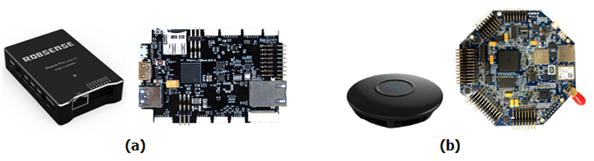
\includegraphics[width=.95\textwidth]{Img/fpga_based}
        \caption{Controlador de vuelo: (a) Phoenix Pro DevKit, (b) OcPoc}
        \label{fig:fpga_based}
    \end{figure}
\end{itemize}

\subsection{Plataformas basadas en ARM MCUs}
\begin{itemize}
    \item \textbf{Pixhawk:} consiste en un controlador PX4-Flight Management Unit (FMU) y una PX4-IO integrada en una misma placa con IO adicionales, memoria y otras características (Fig. \ref{fig:pixhawks}.a). Se encuentra dentro del proyecto DroneCode\footnote{https://www.dronecode.org/}.
    \item \textbf{Pixhawk 2:} Es un cubo pequeño que cuenta con tres IMUs redundantes y hasta tres módulos GPS (Fig. \ref{fig:pixhawks}.b) (Ardupilot). Toda la conección IO del cubo se encuentra en un conector DF17. Su placa portadora posee una interfaz con Intel Edison.
    
    \begin{figure}[!ht]
        \centering
        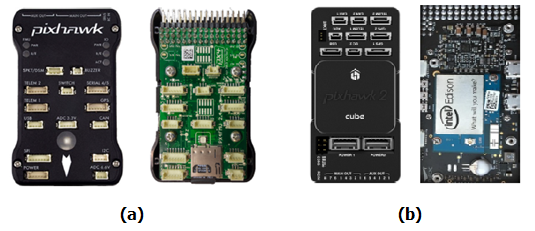
\includegraphics[width=.95\textwidth]{Img/pixhawks}
        \caption{Controlador de vuelo: (a) Pixhawk, (b) Pixhawk 2}
        \label{fig:pixhawks}
    \end{figure}
    
    \item \textbf{FlightCtrl:} Desarrollada por MikroKopter, su última versíon introducida al mercado, la V3.0 (Fig. \ref{fig:flypaparazzi}.a), cuenta con un microcontrolador avanzado, sistema de telemetría, GPS, entre otros, además de ofrecer sistemas con placas de control de vuelo duplicadas que mantienen el helicóptero estable incluso si hay una falla en la placa primaria de control de vuelo.
    \item \textbf{Paparazzi:} Es el primer proyecto de software y hardware open-source para drones. En marzo de 2017 salió el nuevo autopilot del mismo llamado Chimera (Fig. \ref{fig:flypaparazzi}.b) el cual está basado en el microcontrolador STM32F7.
    \item \textbf{FlyMaple:} basada en el Maple Project, el cual es un procesador Arduino ARM, consiste en una placa controladora para cuadricópteros (Fig. \ref{fig:flypaparazzi}.c). La misma cuenta como aplicaciones típícas las de robots balancines, plataformas móbiles, helicópteros y cuadricópteros que requieren IMUs y controladores en tiempo real de alto rendimiento.
    
    \begin{figure}[!ht]
        \centering
        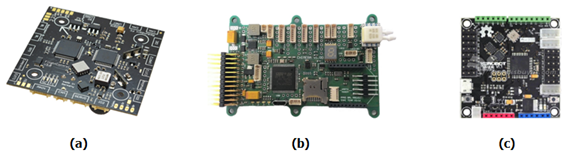
\includegraphics[width=.95\textwidth]{Img/flypaparazzi}
        \caption{Controlador de vuelo: (a) FlightCtrl v3.0, (b) Paparazzi Chimera, (c) FlyMaple}
        \label{fig:flypaparazzi}
    \end{figure}
    
    \item \textbf{CC3D y Atom:} Son dos controladoras de vuelo que poseen las mismas funcionalidades pero con tamaños diferentes. Los mismos (Figs. \ref{fig:apmatom}.a y \ref{fig:apmatom}.b) tienen todos los tipos de hardware de estabilización que corre el firmware OpenPilot/LibraPilot. Pueden ser configuradas para volar con cualquier frame.
    
    \item \textbf{Ardupilot Mega (APM):} Desarrollada por la comunidad DIY Drones como una mejora de la controladora de vuelo Autopilot, consiste en una plataforma basada en  el Arduino Mega (Fig. \ref{fig:apmatom}.c). Puede controlar multicópteros autónomos, helicópteros tradicionales, entre otros.

    \begin{figure}[!ht]
        \centering
        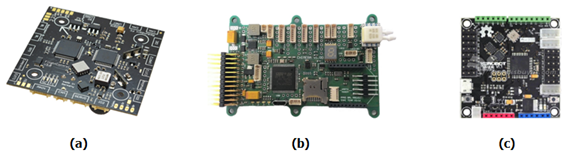
\includegraphics[width=.95\textwidth]{Img/flypaparazzi}
        \caption{Controlador de vuelo: (a) CC3D, (b) Atom, (c) Ardupilot Mega 2.8}
        \label{fig:apmatom}
    \end{figure}
\end{itemize}

\subsection{Plataformas basadas en Raspberry Pi}
\begin{itemize}
    \item \textbf{Erle-Brain 3:} Consiste en un open pilot para drones basado en Linux desarrollado por Erle Robotics (Fig. \ref{fig:raspi}.a). Combina una Raspberry Pi junto a PXFmini, contando esta última con sensores, IO y alimentación. Está diseñado sobre el proyecto DroneCode.
    \item \textbf{NAVIO2 Autopilot:} Es una integración de sensores, GPS y alimentación apareado con una Raspberry Pi. Cuenta con doble IMU para mejorar el desempeño y conseguir redundancia (Fig. \ref{fig:raspi}.b).
    
    \begin{figure}[!ht]
        \centering
        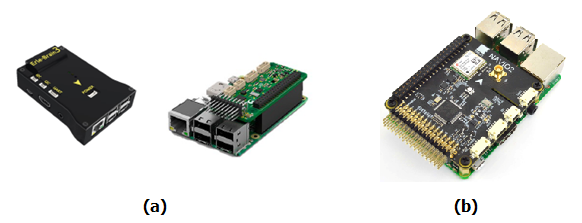
\includegraphics[width=.95\textwidth]{Img/raspi}
        \caption{Controlador de vuelo: (a) Erle-Brain 3 Autopilot, (b) NAVIO2 Autopilot}
        \label{fig:raspi}
    \end{figure}
\end{itemize}

\subsection{Plataformas basadas en Qualcomm}
\begin{itemize}
    \item \textbf{Snapdragon Autopilot:} la plataforma Snapdragon Flight (Fig. \ref{fig:snapdragon}) es un piloto automático de gama alta que puede ejecutar el plan de vuelo sobre un sistema operativo en tiempo real DSP utilizando la API DSPAL para la compatibilidad con POSIX. El mismo cuenta con un SoC Snapdragon 801. En comparación con la Pixhawk, sus características incluyen potencia de procesamiento avanzada, control de vuelo en tiempo real en Hexagon DSP, Wi-Fi, conectividad Bluetooth, GPS automotriz, una cámara de flujo óptico y una cámara de video de resolución 4K.    
    \begin{figure}[!ht]
        \centering
        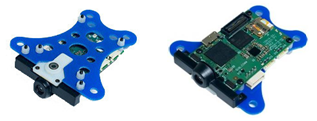
\includegraphics[width=.55\textwidth]{Img/snapdragon}
        \caption{Snapdragon Flight}
        \label{fig:snapdragon}
    \end{figure}
\end{itemize}

\subsection{Comparación entre plataformas existentes}


En el Cuadro \ref{tab:plataformas} \cite{yang2016}\cite{raj2016} se resumen las características principales. En la misma, se observa que la principal diferencia entre ellas es la unidad de procesamiento, además de que no todas ellas presentan redundancia de sensores críticos.

% Please add the following required packages to your document preamble:
% \usepackage{booktabs}
% \usepackage{graphicx}
\begin{table}
\resizebox{\textwidth}{!}{%
\begin{tabular}{@{}|c|c|c|c|c|c|c|@{}}
\toprule
\textbf{Plataforma} & \textbf{Procesador} & \textbf{Sensores} & \textbf{\begin{tabular}[c]{@{}c@{}}Interfaces /\\ Conectividad\end{tabular}} & \textbf{Redundancia} & \textbf{\begin{tabular}[c]{@{}c@{}}Dimensiones \\ (mm)\end{tabular}} & \textbf{Peso (g)} \\ \midrule
Phoenix Pro & \begin{tabular}[c]{@{}c@{}}Xilinx Zynq\\ 7020\end{tabular} & \begin{tabular}[c]{@{}c@{}}Acelerometro,\\ giroscopo,\\ barómetro,\\ GPS\end{tabular} & \begin{tabular}[c]{@{}c@{}}USB, UART, I2C,\\ CAN, SPI, miniHDMI,\\ Camera Link, LVDS,\\ PWM, telemetria\end{tabular} & - & 73,8*55,8*18 & 64 \\ \midrule
OcPoc & \begin{tabular}[c]{@{}c@{}}Xilinx Zynq\\ Z-7010\end{tabular} & \begin{tabular}[c]{@{}c@{}}IMU 9 DOF\\ (MPU9250),\\ Barometro\\ (MS5611)\end{tabular} & \begin{tabular}[c]{@{}c@{}}I2C, USB-OTG,\\ USB-UART, SPI, \\ CSI, GSI, CAN, \\ ADC, PWM\end{tabular} & \begin{tabular}[c]{@{}c@{}}IMU\\ (MPU9250)\end{tabular} & 92*64*21 & 70 \\ \midrule
PIXHAWK & \begin{tabular}[c]{@{}c@{}}ARM\\ Cortex-M4F\end{tabular} & \begin{tabular}[c]{@{}c@{}}Giroscopo\\ (L3GD20H),\\ acelerometro /\\ magnetometro\\ (LSM303D),\\ barometro\\ (MS5611)\end{tabular} & \begin{tabular}[c]{@{}c@{}}UART, CAN, I2C,\\ SPI, ADC, PWM\end{tabular} & \begin{tabular}[c]{@{}c@{}}Giroscopo /\\ acelerometro \\ (MPU6000)\end{tabular} & 50*15,5*81,5 & 38 \\ \midrule
PIXHAWK2 & \begin{tabular}[c]{@{}c@{}}ARM\\ Cortex-M4F\end{tabular} & \begin{tabular}[c]{@{}c@{}}IMU 9 DOF\\ (MPU9250 /\\ ICM20948 /\\ ICM20648 /\\ L3GD20 +\\ LSM303D), \\ Barometro\\ (MS5611)\end{tabular} & \begin{tabular}[c]{@{}c@{}}S.Bus, I2C, SPI, \\ CAN, Carrier board \\ para Intel\\ Edison, ADC, \\ PWM\end{tabular} & \begin{tabular}[c]{@{}c@{}}2x IMU \\ (MPU9250),\\ Barometro\\ (MS5611)\end{tabular} & \begin{tabular}[c]{@{}c@{}}50*15,5*81,6\\ +35*35 (Cube)\end{tabular} & - \\ \midrule
FlightCtrl V3.0 & \begin{tabular}[c]{@{}c@{}}ARM\\ Cortex-M4F\end{tabular} & \begin{tabular}[c]{@{}c@{}}Giroscopo,\\ magnetometro,\\ acelerometro,\\ barometro, GPS\end{tabular} & \begin{tabular}[c]{@{}c@{}}UART, I2C, SPI, \\ ADC, PWM, S.Bus, \\ CAN, telemetria\end{tabular} & - & 67*67*- & 32 \\ \midrule
Paparazzi & STM32F767 & \begin{tabular}[c]{@{}c@{}}IMU 9 DOF\\ (MPU9250),\\ Barometro\\ (MS5611),\\ Sensor de \\ presion\\ (MS4525DO)\end{tabular} & \begin{tabular}[c]{@{}c@{}}UART, I2C, SPI, \\ CAN, USB, PWM,\\ PPM/S.Bus\end{tabular} & - & 89*60*- & - \\ \midrule
CC3D/Atom & STM32F & \begin{tabular}[c]{@{}c@{}}Giroscopio /\\ acelerometro \\ (MPU6000)\end{tabular} & \begin{tabular}[c]{@{}c@{}}UART, I2C,\\ S.Bus/PPM, PWM\end{tabular} & - & \begin{tabular}[c]{@{}c@{}}36*36*-(CC3D)\\ 15*7*- (Atom)\end{tabular} & \begin{tabular}[c]{@{}c@{}}8 (CC3D)\\ 4 (Atom)\end{tabular} \\ \midrule
APM & ATMEGA2560 & \begin{tabular}[c]{@{}c@{}}Giroscopo /\\ acelerometro \\ (MPU6000),\\ barometro(MS5611), \\ GPS\end{tabular} & \begin{tabular}[c]{@{}c@{}}I2C, PWM, UART, \\ OSD, telemetria\end{tabular} & - & 142*96*18 & 55 \\ \midrule
FlyMaple & STM32F103 & \begin{tabular}[c]{@{}c@{}}Giroscopo\\ (ITG-3200),\\ acelerometro\\ (ADXL345),\\ magnetometro\\ (HMC5883L),\\ barometro\\ (BMP085), GPS\end{tabular} & \begin{tabular}[c]{@{}c@{}}PWM, USB, UART, \\ I2C, ADC\end{tabular} & - & 50*50*12 & 15 \\ \midrule
Erle-Brain 3 & \begin{tabular}[c]{@{}c@{}}ARMv8\\ Quad-Core\\ (Raspberry PI 3)\end{tabular} & \begin{tabular}[c]{@{}c@{}}Giroscopo,\\ magnetometro,\\ acelerometro,\\ barometro, GPS,temperatura\end{tabular} & \begin{tabular}[c]{@{}c@{}}I2C, UART, USB, \\ HDMI, Ethernet, PWM, \\ PPM/S.Bus,ADC, \\ Bluetooth, Audio Jack\end{tabular} & - & 95*70*23,8 & 100 \\ \midrule
NAVIO2 & \begin{tabular}[c]{@{}c@{}}ARMv8\\ Quad-Core\\ (Raspberry PI 3)\end{tabular} & \begin{tabular}[c]{@{}c@{}}IMU 9 DOF \\ (MPU9250), \\ barometro, \\ GPS, RC I/O\end{tabular} & \begin{tabular}[c]{@{}c@{}}I2C, UART,\\ PWM, S.Bus\end{tabular} & \begin{tabular}[c]{@{}c@{}}IMU 9 DOF\\ (LSM9DS1)\end{tabular} & 55*65*- (shield) & 23 (shield) \\ \midrule
Snapdragon & \begin{tabular}[c]{@{}c@{}}Snapdragon\\ 801\end{tabular} & \begin{tabular}[c]{@{}c@{}}IMU 9 DOF\\ (MPU9250),\\ barometro\\ (BMP280),\\ optical flow\\ (OV7251), GPS\end{tabular} & \begin{tabular}[c]{@{}c@{}}Wifi, USB, PWM, \\ UART, I2C\end{tabular} & - & 68*52*- & - \\ \bottomrule
\end{tabular}%
}
\caption{Comparativa entre distintas plataformas disponibles}
\label{tab:plataformas}
\end{table}

En muchas de las plataformas analizadas, puede observase la presencia de sensores duplicados, tal como es el caso de giroscopos y acelerómetros. Dicha \textit{redundancia} permite al sistema aumentar su \textit{confiabilidad}, logrando así reducir las posibles fallas del sistema, sobre todo en los sensores más críticos \cite{petritoli2018}\cite{dhillon1991}.

\subsection{Estándar de Hardware}

A partir del relevamiento realizado, se puede establecer que los métodos de conexión que presentan las plataformas existentes en el mercado no cuentan con un estándar de hardware definido, sino que cada una tiene su interfaz de conexión propia. Esto trae como inconveniente que, si se requiere expandir su funcionalidad agregando, por ejemplo, más sensores, en base a la plataforma que se tenga dependerá el hardware asociado a realizarse.

\subsubsection{PC/104}
PC/104 es una familia de estándares de computadoras embebidas que definen tanto los factores de forma como los buses de sistema. El mismo está diseñado para entornos especializados donde se requiere un sistema informático pequeño y resistente. El estándar es modular, permitiendo \textit{stackear} placas de una gran variedad de fabricantes con tal de producir un sistema integrado personalizado \cite{pc104}.

Las placas PC/104 se apilan unas sobre otras como bloques de construcción. La especificación PC/104 define cuatro orificios de montaje en las esquinas de cada módulo, lo que permite que las tablas se sujeten entre sí mediante separadores. El tamaño de la placa compacta contribuye aún más a la robustez del factor de forma al reducir la posibilidad de flexión de PCB bajo impacto y vibración.

\begin{figure}[!ht]
    \centering
    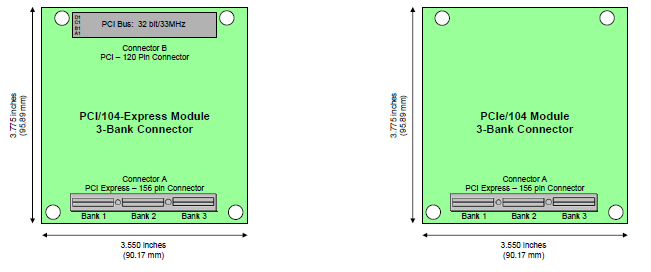
\includegraphics[width=\textwidth]{Img/pci104threebank}
    \caption{Board Layouts de PCI/104-Express y PCIe/104}
    \label{fig:pci104threebank}
\end{figure}

Las estructuras de buses definidos son los que dan lugar a las familias de estándares conocidos del mismo, siendo:

\begin{itemize}
    \item \textbf{PC/104:} Este bus original deriva del bus ISA. Incluye todas las señales encontradas en el mismo, con pines de tierra adicionales agregados para garantizar la integridad del bus.
    \item \textbf{PC/104-Plus:} El mismo agrega soporte para el bus PCI, además del bus ISA del estándar PC/104.
    \item \textbf{PCI-104:} Incluye el conector PCI, pero no el conector PC/104, para aumentar el espacio disponible de la placa. A pesar de que el conector PCI tiene 120 pines en lugar de 104, se mantuvo el nombre establecido. La ubicación del conector PCI y el pinout son idénticos a PC/104-Plus. Dado que se omite el bus ISA, una placa PCI-104 es incompatible con el módulo periférico PC/104. Sin embargo, PCI-104 y PC/104-Plus son compatibles, ya que ambos utilizan el bus PCI. La mayoría de las placas PC/104-Plus pueden fabricarse como PCI-104 simplemente no rellenando el conector PC/104. PCI-104 utiliza el mismo esquema de selección de Número de Ranura PCI que PC/104-Plus. Cada dispositivo debe asignarse a un número de ranura único.
    \item \textbf{PCI/104-Express:} Incorpora el bus PCI Express (PCIe) además del bus PCI de la generación anterior. La especificación define un conector de montaje en superficie de 156 pines para las señales PCI Express. El nuevo conector ocupa la misma ubicación de la placa que el conector ISA PC/104 heredado. Además de PCI Express, las especificaciones también definen los pines en el conector para buses modernos adicionales, como USB y SATA.
    \item \textbf{PCIe/104:} Similar al estándar PCI/104-Express, pero omite el bus PCI heredado para aumentar el espacio disponible en la placa (similar a la relación entre PC/104-Plus y PCI-104). La ubicación del conector PCI Express y las opciones de asignación de patillas son las mismas que para PCI/104-Express (Tipo 1 y Tipo 2). Debido a que se omite el conector de bus PCI, una placa PCIe/104 es incompatible con los sistemas PC/104-Plus y PCI-104 (a menos que se use un dispositivo de puente PCIe a PCI).
\end{itemize}

El factor de forma 104 define el tamaño de la placa (90 * 96 mm), con orificios de montaje en las cuatro esquinas de la placa. Las especificaciones también permiten un área de 0.5 pulgadas (13 mm) más allá del borde de la PCB para los conectores de entrada y salida. La especificación PCI/104-Express y PCIe/104 introdujo el nombre ''104'' para distinguir el factor de forma del bus PC/104 heredado. A su vez, dichas especificaciones aceptan las opciones de uno (Fig. \ref{fig:pci104threebank}) o tres (Fig. \ref{fig:pci104onebank}) \textit{bancos}, agregando mayor flexibilidad al diseñador \cite{pci104express}.

\begin{figure}[!ht]
    \centering
    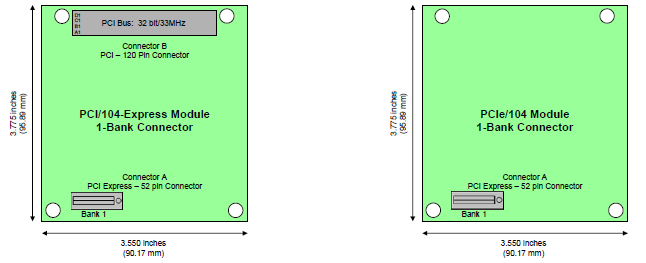
\includegraphics[width=\textwidth]{Img/pci104onebank}
    \caption{Board Layouts de PCI/104-Express y PCIe/104 con conector OneBank}
    \label{fig:pci104onebank}
\end{figure}
    
